% !TEX root = ../tesi.tex
%
\chapter{High Energy Nuclear Physics}
\label{sec:1}

\cleanchapterquote{Three quarks for Muster Mark! \\
                    Sure he has not got much of a bark\\
                    And sure any he has it's all beside the mark.}{James Joyce}{(Finnegans Wake)}

% \cleanchapterquote{The universe has been expanding since the big bang, thus early on it was hot and dense. To trace the history of the universe we must understand the dynamics that operates when the universe was hot and particles were very energetic. }{David Gross}{Nobel Lecture}

According to cosmological theories, in its early stages the Universe was extremely hot and dense.
In the first few microseconds, the energy densisty was so high that hadrons could not be formed and
their foundamental constituents were in a deconfined state. When the energy density has decreased
enough, a phase transition led to the formation of the ordinary matter. 

High Energy Nuclear Physics (HENP) investigates the hot and dense nuclear matter and the properties
of its phase ransition into ordinary matter through the study of ultra-relativistic heavy-ion collisions. 
The aim is to improve our understandig of the behaviour of the matter in extereme conditions and of the
Universe at the beginning of its life.

\section{QCD: the theory of the Strong Interaction}
\label{sec:1.1}

In 1964 M. Gell-Mann and G. Zweig proposed independently a model that could explain the existence of
the great variety of hadrons discovered in the 1950s and 1960s \cite{gellmann, zweig1, zweig2}. 
This model, known as the Static Quark Model, was based on the assumption that hadrons are not
fundamental particles, but they are composed states of elementary constituents called quarks.
In this way it was possible to explain the large number of particles observed and their properties,
which showed some sort of pattern, in term of constituents properties.
Furthermore, thanks to the Static Quark Model, it was possible predict new hadrons (e.g. 
$\Omega^{-}\xspace$) and to explain why certain particles don't exist (e.g. baryons with $S=+1$).
However, this model could not deal with many questions: why there is no evidence of free quarks?
What hold quarks together in a hadron? Why the $\Delta^{++}$ baryon exists despite is forbidden
by Pauli's Principle?
In order to answer these questions it was necessary to introduce a new quantum number the colour
\cite{fritzsch-gellmann}. The introduction of the colour led to the formulation of a quantum field theory
for the Strong Interaction, inspired by the Quantum Electrodynamics (QED), the Quantum Chromodynamics
(QCD).

The QCD is a non-Abelian quantum gauge theory, based on the invariance under local $\mathrm{SU(3)}_{c}$ 
group transformations. The choice of this particular symmetry group is due to the hypothesis
that the colour comes in three different states: red, blue and green.
The local invariance under $\mathrm{SU(3)}_{c}$ implies the existence of 8 massless gauge bosons
mediators of the colour interaction, called gluons \cite{fr-gm-hl-gluons}.
Therefore the QCD Lagrangian can be written as:
\begin{equation}
    \Lagr_{\mathrm{QCD}} = \bar{\psi_{i}}(i(\gamma^{\mu}D_{\mu})_{ij}-m\delta_{ij})\psi_{j} 
    - \frac{1}{4}G^{a}_{\mu \nu} G^{\mu \nu}_{a}
\end{equation}
where the first term is related to quarks fields while the second is releted to gluons fields.
In the first term $\psi_{i}(x)$ represents the quarks fields expressed in the fundamental 
representation of $\mathrm{SU(3)}_{c}$, while $D_{\mu}$ is the covariant derivative, defined as:
\begin{equation}
    D_{\mu} = \partial_{\mu} - ig_{s}A^{a}_{\mu}\lambda_{a}.
\end{equation}
In this derivarives shows up the coupling constant for the Strong Interaction $g_{s}$, the 
Gell-Mann matrices $\lambda_{\alpha}$ which gives a representation of the generators of 
$\mathrm{SU(3)}_{c}$ symmetry group, and the gluon field $A(x)$.
This first term of the QCD Lagrangian represents the quarks-gluons interaction via a 
QED-like vertex.

\vspace{1cm}
\begin{figure}[!h]
\captionsetup{justification=centering}
\centering
    \begin{fmffile}{2gluoni1quark}
        \begin{fmfgraph*}(80,60)
            \fmfleft{i1}
            \fmfright{o1,o2}
            \fmf{gluon}{i1,v1}
            \fmf{fermion}{o1,v1,o2}
            \fmflabel{$a$}{i1}
            \fmflabel{$\psi_i$}{o1}
            \fmflabel{$\psi_j$}{o2}
        \end{fmfgraph*}
    \end{fmffile}
\vspace{1cm}
\caption{Feynman diagram for the gluon-quarks interaction.}
\end{figure}

The second term of the Lagrangian $G^{a}_{\mu \nu}$ represents the gauge invariant gluon field 
strength tensor, and can be written as:
\begin{equation}
    G^{a}_{\mu \nu} = \partial_{\mu} A^{a}_{\nu} - \partial_{\nu} A^{a}_{\mu} + 
    g_{s} f^{abc} A^{b}_{\mu} A^{c}_{\nu}.
\end{equation}
In this tensor $g_{s} f^{abc} A^{b}_{\mu} A^{c}_{\nu}\ $ is the non-Abelian part of the theory, 
which implies the self-interactions among gluons. This interactions have resulted from the
fact that gluons carry a colour and an anti-colour charge, so they can interact among themselves.
Therefore in addition to the QED-like vertex, in the QCD, 3 gluons and 4 gluons vertex are allowed
at the tree level. 
The existence of the gluons vertex allows to have gluons loops.

\vspace{1cm}
\begin{figure}[!h]
    \hspace{2cm}
    \begin{fmffile}{3gluoni}
        \begin{fmfgraph*}(80,60)
            \fmfleft{i1}
            \fmfright{o1,o2}
            \fmf{gluon}{i1,v1}
            \fmf{gluon}{o1,v1,o2}
            \fmflabel{$a,\mu$}{i1}
            \fmflabel{$b,\nu$}{o1}
            \fmflabel{$c,\rho$}{o2}
        \end{fmfgraph*}
    \end{fmffile}

    \vspace{-2.1cm}
    \hspace{8cm}
    \begin{fmffile}{4gluoni}
        \begin{fmfgraph*}(80,60)
            \fmfleft{i1,i2}
            \fmfright{o1,o2}
            \fmf{gluon}{i1,v1,i2}
            \fmf{gluon}{o1,v1,o2}
            \fmflabel{$a,\mu$}{i1}
            \fmflabel{$b,\nu$}{i2}
            \fmflabel{$c,\rho$}{o1}
            \fmflabel{$d,\sigma$}{o2}
        \end{fmfgraph*}
    \end{fmffile}
\vspace{1cm}
\caption{Feynman diagrams for the gluon-gluon interactions at the tree level.}
\end{figure}

In the renormalization process of the theory, the non-Abelian nature of the QCD brings to the 
so-called \textit{anti-screening} in colour interaction.
%, since gluons loops have to be considered.
%Indeed, 
Adding loop corrections to the gluons propagator, gluons loops contribute to the sum with
opposite sign respect to the quarks loops.
Therefore, in addition to the QED-like \textit{screening} effect, there is an 
\textit{anti-screening} effect due to gluons loops.
As a result, the QCD shows up its specific features, \textit{asymptotic freedom} and 
\textit{confinement}.

Setting $\alpha_{s} = g^{2}_{s}/4\pi\ $ strong coupling constant can be written as \cite{pdg}:
\begin{equation} \label{eq:alphastrong1}
    \alpha_{s}(Q^{2}) = \frac{\alpha_{s}(\mu^{2})}{1 + \alpha_{s}(\mu^{2})(33 - 2 n_{f})
    \ln(Q^{2}/\mu^{2})}
\end{equation}
where $n_{f}\ $ is the number of quark families and $\mu\ $ is the renormalization scale of 
the theory.
For high transferred momenta $\alpha_{s}\ $ goes to zero and the QCD becomes a free theory and 
this regime is called \textit{asymptotic freedom}. At low $Q^{2}\ $ the Strong copuling diverges,
forcing quarks to be strongly bound in hadrons: the so-called \textit{confinement} regime. 
This behaviour of the QCD copuling constant has been confirmed by experimental results over the
years as shown in Figure \ref{fig:alpharun}.
The equation \ref{eq:alphastrong1} can be rewritten fixing the energy scale:
\begin{equation} \label{eq:alphastrong2}
    \alpha_{s}(Q^{2}) = \frac{12 \pi}{(33 - 2 n_{f})\ln(Q^{2}/\Lambda_{\mathrm{QCD}})}
\end{equation}
where $\Lambda_{\mathrm{QCD}}$ is the renormalization scale of QCD (typically $\approx 200$ MeV).

\begin{figure}[]
    \captionsetup{justification=centering}
    \centering
    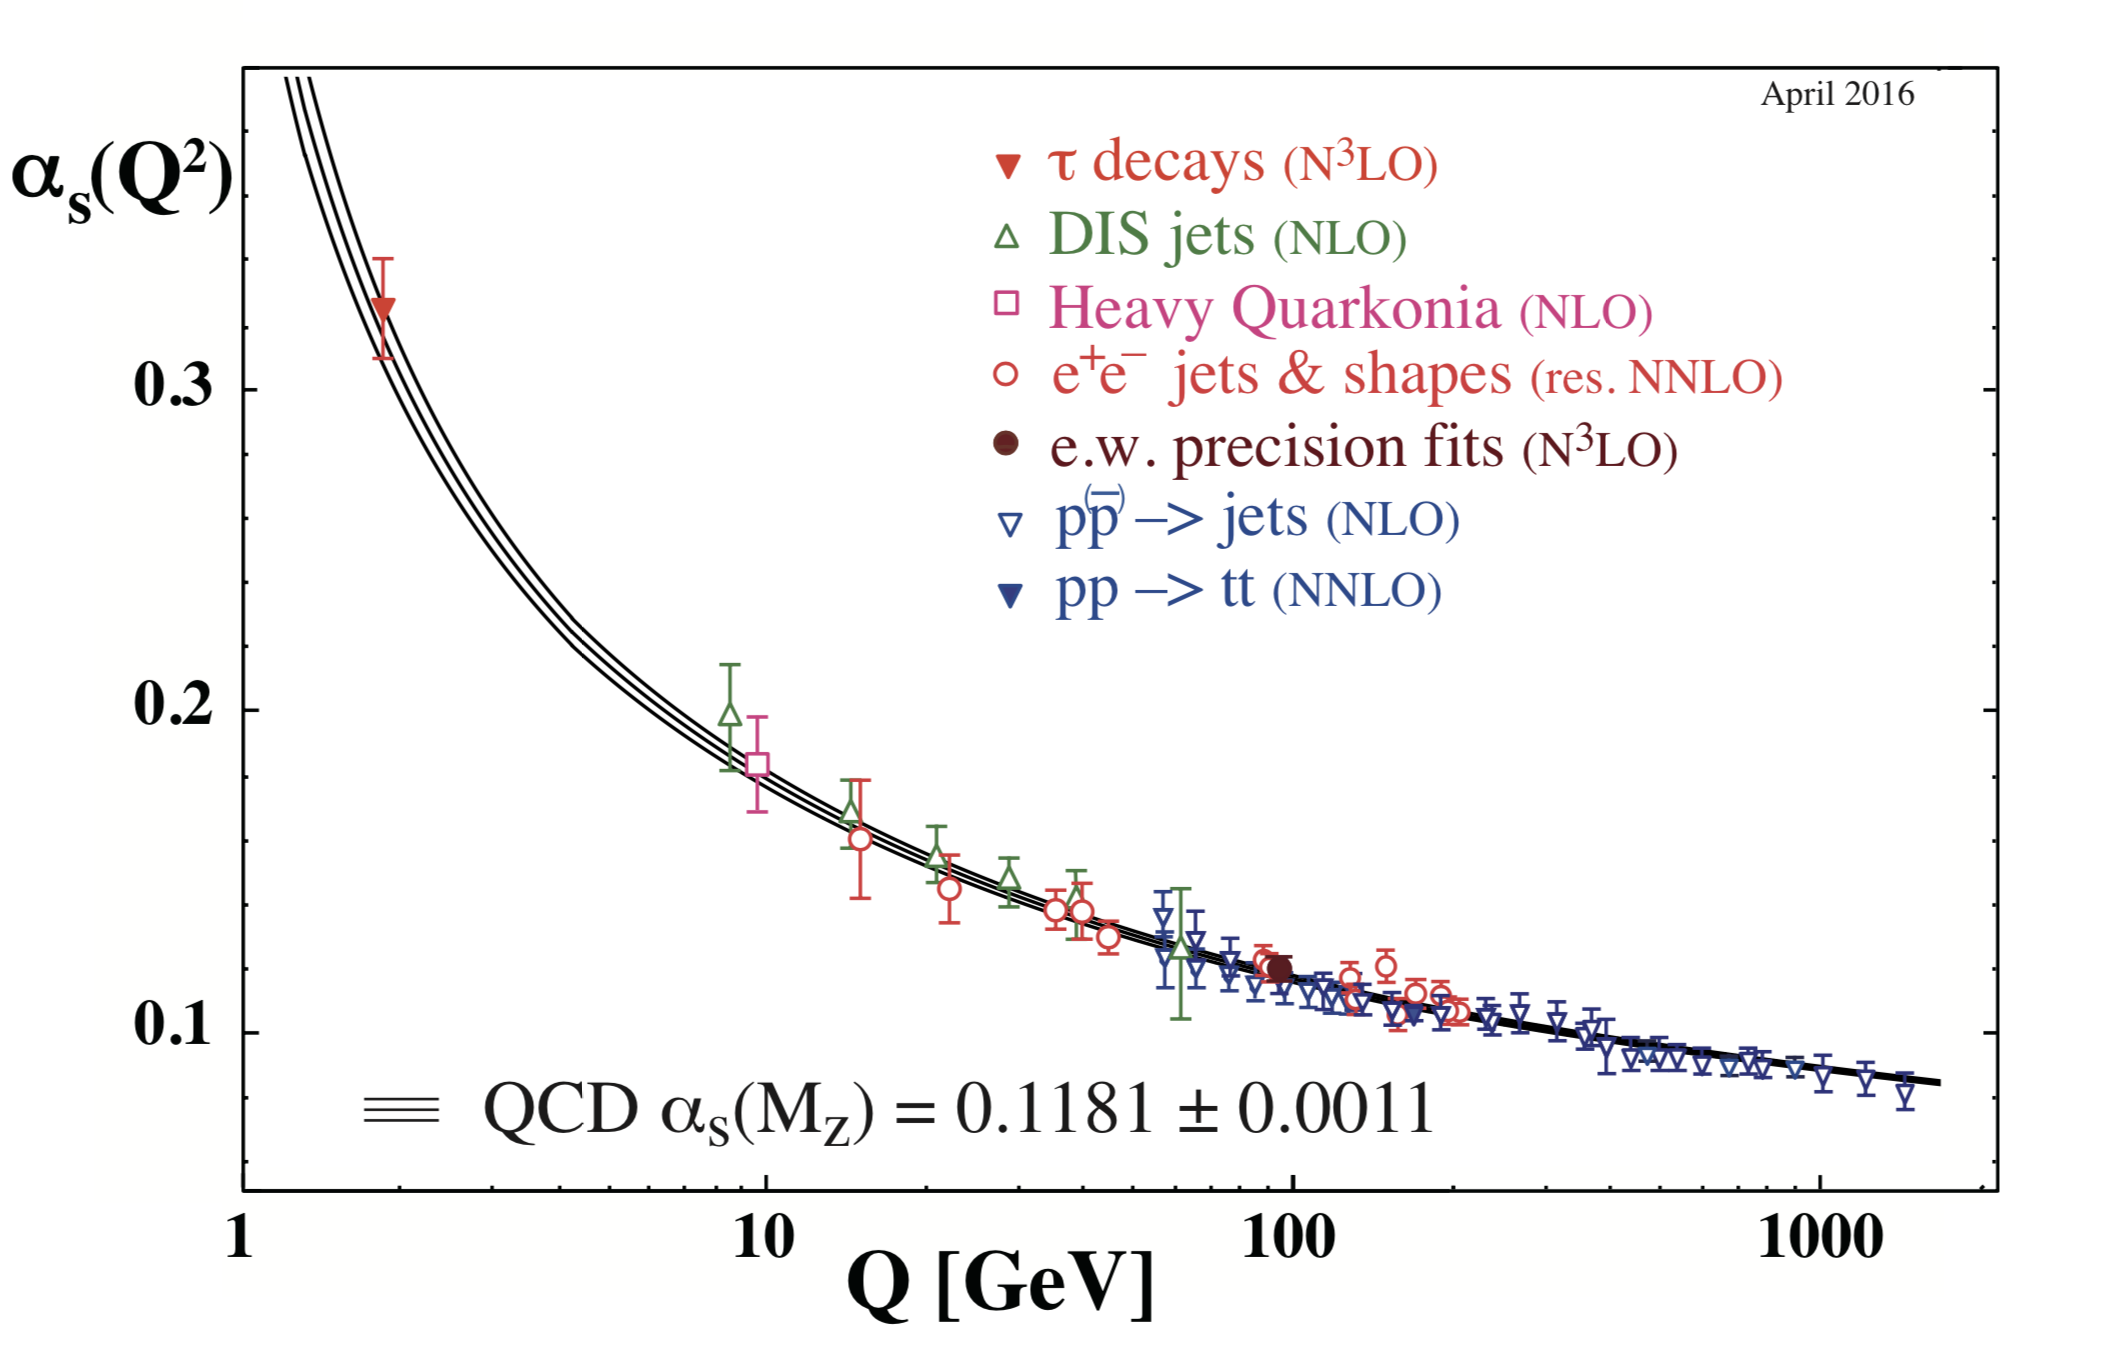
\includegraphics[width=0.8\textwidth]{gfx/alpharun}
	\caption{Summary of measurements of $\alpha_{s}$ as a function of the energy scale $Q$ \cite{pdg}.}
	\label{fig:alpharun}
\end{figure}

In QCD the perturbative approach used to calculate the elements of the scattering matrix (pQCD), is 
possible only for high $Q^{2}\ $ processes ($Q^{2} \gg \mu^{2}$, thus $\alpha_{s} \ll 1$).
As already mentioned, in low transferred momentum processes $\alpha_{s}$ diverges. 
Therefore, is impossible to express the elements of the scattering matrix in terms of power series
expansion of the Strong copuling constant.
In this regime it is still possible to evaluate the Green’s functions of the QCD Lagrangian
on a space-time lattice with spacing a, as proposed in 1974 by Wilson \cite{lattice}.
With this method, called lattice QCD (LQCD) is possible to extrapolate to the continuum 
($a \rightarrow 0$) and get results to be compared with the experiments.

%
%
\section{States of hadronic matter}
\label{sec:1.2}

One of the interesting consequences of the running copuling constant is the possibility of having
different states of the hadronic matter. The state is essentially determined by the mean transferred 
momentum in the interactions which define the value of $\alpha_{s}$. 
A system with low mean transferred momentum it is in the \textit{confinement} regime, therefore quarks
and gluons are required to be confined in hadrons. Otherwise in high mean transferred momentum systems,
the \textit{asymptotic freedom} regime allows the formation of a plasma where quarks and gluons are
essentially free. This state of matter is called Quark Gluon Plasma (QGP) and is supposed that the 
universe was in this state in the first microseconds after the Big Bang.
One of the main goals of the HENP is the study of the phase transitions between the different
states of the hadronic matter.

Considering a system with finite dimensions, composed by hadronic matter, can be useful to describe it 
using thermodinamical variables like temperature $(T)$ and chemical potential $(\mu)$. In this
specific framework the chemical potential is interpreted as the energy required to create a 
baryonic state and it is called baryon chemical potential $(\mu_{B})$. 
Figure \ref{fig:qgpdiagram} shows the phase diagram of the QCD matter predicted by the theory and 
the values of temperature $T$ and baryon chemical potential $(\mu_{B})$ which are accessible
experimentally in high energy heavy ion collisions.

\begin{figure}[]
    \centering
    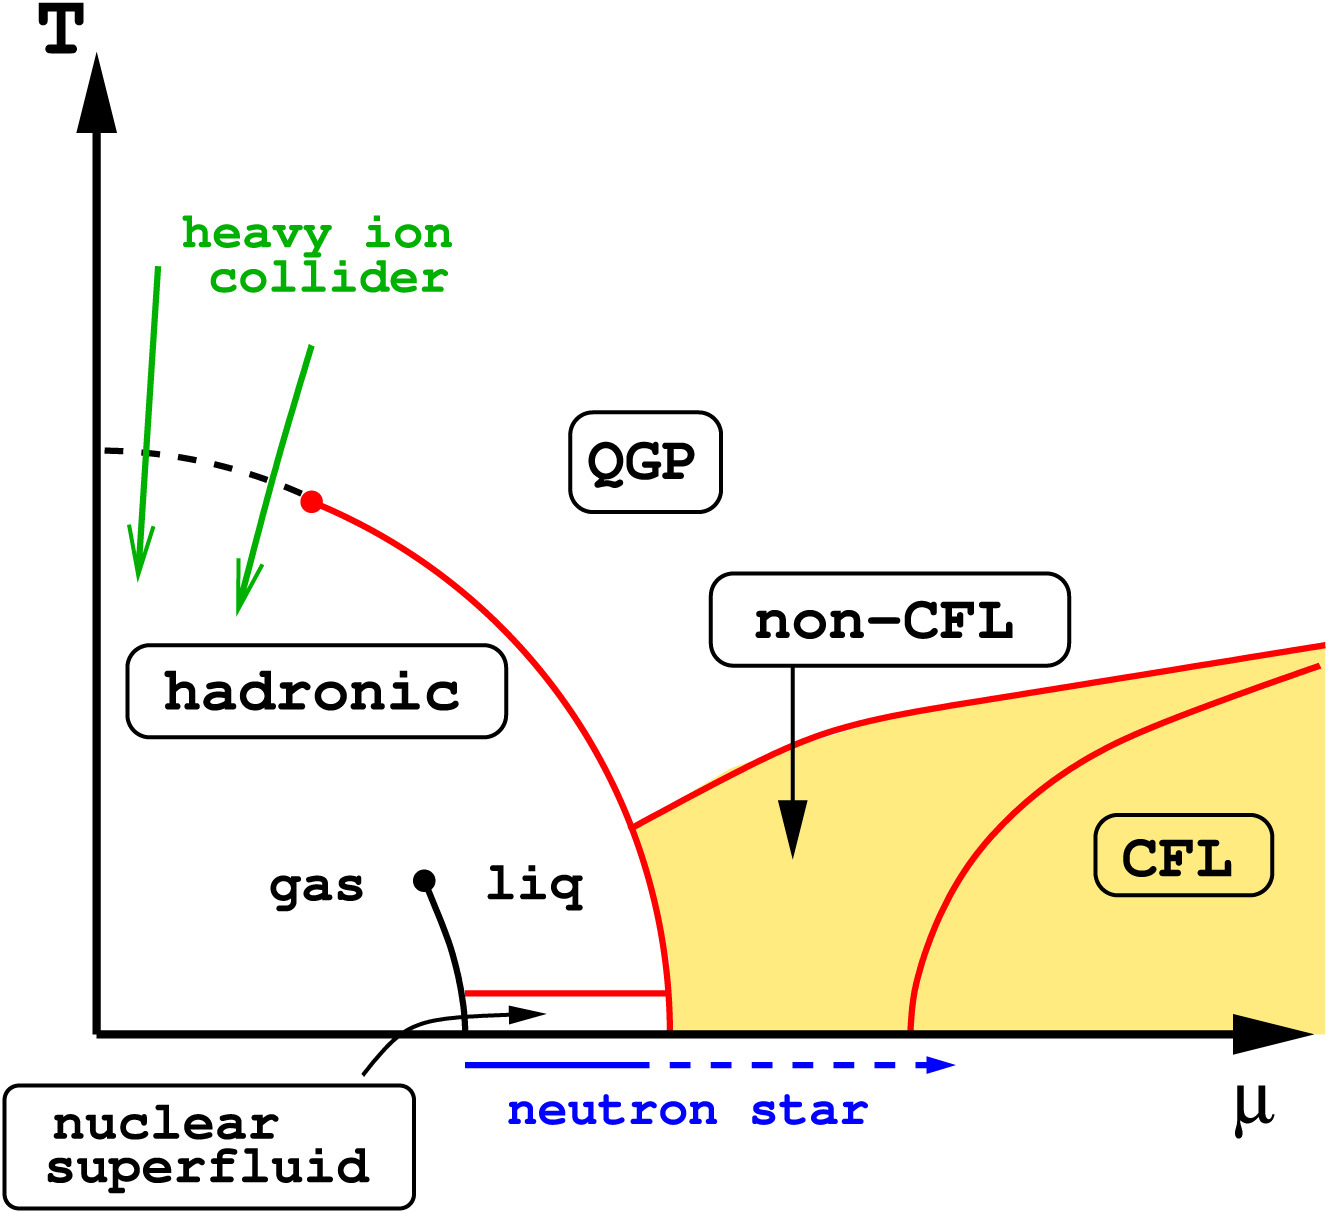
\includegraphics[width=0.6\textwidth]{gfx/qgpphase}
	\caption{Schematic representation of the nuclear matter phase diagram from \cite{qgpphase}. QGP refers to the Quark Gluon Plasma state, CFL (Colour-Flavour Locked) corresponds to the colour superconducting phase that is present in systems with high baryon chemical potential. The green arrows represent the phase space investigated by collider experiments at the Relativistic Heavy Ion Collider (RHIC) and at the LHC.}
	\label{fig:qgpdiagram}
\end{figure}

The origin of the diagram (T$=\mu_{B}=0$ GeV) corresponds to the QCD vacuum. At T$=0$ GeV, $\mu_{B}$ is 
the energy required to create a baryonic state, therefore ordinary matter (proton, neutrons and nuclei)
sits around $1$ GeV on the $\mu_{B}$ axis. Along the $\mu_{B}$ axis lies a phase transition to a state,
the Color Superconducting Phase, that has been hypothesised to be present in matter at high density,
e.g. in  the core of neutron stars \cite{csp}.
Along the T axis, where $\mu_{B}=0$, there is a phase transition when T$\ \gg \Lambda_{\mathrm{QCD}}$. 
At this temperatures the average momentum exchange between quarks and gluons is so high that they reach
the \textit{asymptotic freedom}, hence they are no longer confined in colour singlets states.
In these conditions they constitute a plasma of free coloured partons, similar to the primordial 
universe: the aforementioned QGP.

The order of the phase transition is determined by the behaviour of the derivatives of the free energy
of the system with respect to time. It basically describes how fast the free energy varies in a 
neighbourhood of the transition temperature.
A first order transitions takes place when a latent heat is present, leading to a discontinuous free
energy first derivatives and variation of entropy.
If no latent heat is involved in the process, occours a second order transition. The free energy 
first derivative is continuous, while derivatives of higher than first order of the free energy are 
discontinuous.
When the transition occours with a continuous behaviour of the free energy and its derivatives,
it is called a \textit{crossover} transition.
In $\mu_{B}=0$ conditions, the transition from hadron gas to the QGP takes place when T $\approx 150$ MeV
with a \textit{crossover} transition.

%
%
\section{Heavy Ion Collisions}
\label{sec:1.3}

The QCD phase diagram is derived by theories and models, but their predictions are difficult to test.
For the T $\approx0$ GeV and high $\mu_{B}$ region, important suggestions can come from astronomic observations 
of neutron stars. 
For high T regions, instead, the only known way to cross the phase boundary between ordinary hadronic matter
and QGP is by colliding ultrarelativistic heavy ions in the laboratory.

The journey of the High Energy Nuclear Physics started in the '70 at the Lawrence Berkeley National Laboratory
where the first experiments on heavy ions collisions (HIC) was performed at modestly relativistic conditions 
($\approx 2\ $ GeV/nucleon).
In 1986, two HIC experiments started simultaneously at the Super Proton Syncrotron (SPS) at CERN and at the
Alternate Gradient Syncrotron (AGS) at Brookhaven, colliding O ions at fixed target at higher energies.
Nowdays the two main hadron colliders active with an HIC program and dedicated experiments are the
Relativistic Heavy Ion Collider (RHIC) at the Brookhaven National Laboratory (BNL) and the Large Hadron
Collider (LHC) at CERN.

\subsection{The "Little Bang" at the LHC}
\label{sec:1.3.1}

Atomic nuclei are composite systems of nucleons with finite dimensions. When they collide at 
ultrarelativistic energies the problem of the description of the collision, that can be very
complex, arises.
The Glauber Model \cite{glauber} is a semi-classical model describing nucleus–nucleus 
interaction in terms of nucleon–nucleon (NN) interactions.
The Glauber Model is based on the assumption of the \textit{optical limit}:
\begin{itemize}
    \item nucleons are point like and independent inside the nuclei;
    \item only hadronic interactions are considered: protons and neutrons cannot be distinguished;
    \item the collision does not deflect colliding nucleons: they travel in a straight line;
    \item the cross section for an elementary nucleon-nucleon interaction is constant during the whole 
    process.
\end{itemize}
With this assumption the Glauber Model allows a quantitative calculation of the interaction
probability, the number of elementary NN collisions ($\mathrm{N}_{coll}$), the number
of the partecipants nucleons ($\mathrm{N}_{part}$) and extension of the overlap region.
These quantities are expressed in terms of the impact parameter $\vec{b}$, which characterizes
the collisions geometry.
A direct experimental measurement of the impact parameter is precluded and the same goes for
$\mathrm{N}_{coll}$ and $\mathrm{N}_{part}$.
However, the Glauber Model enables to correlate this variables with measurable quantities
such as the total number of particles produced in the collision.

\begin{figure}[!h]
    \centering
    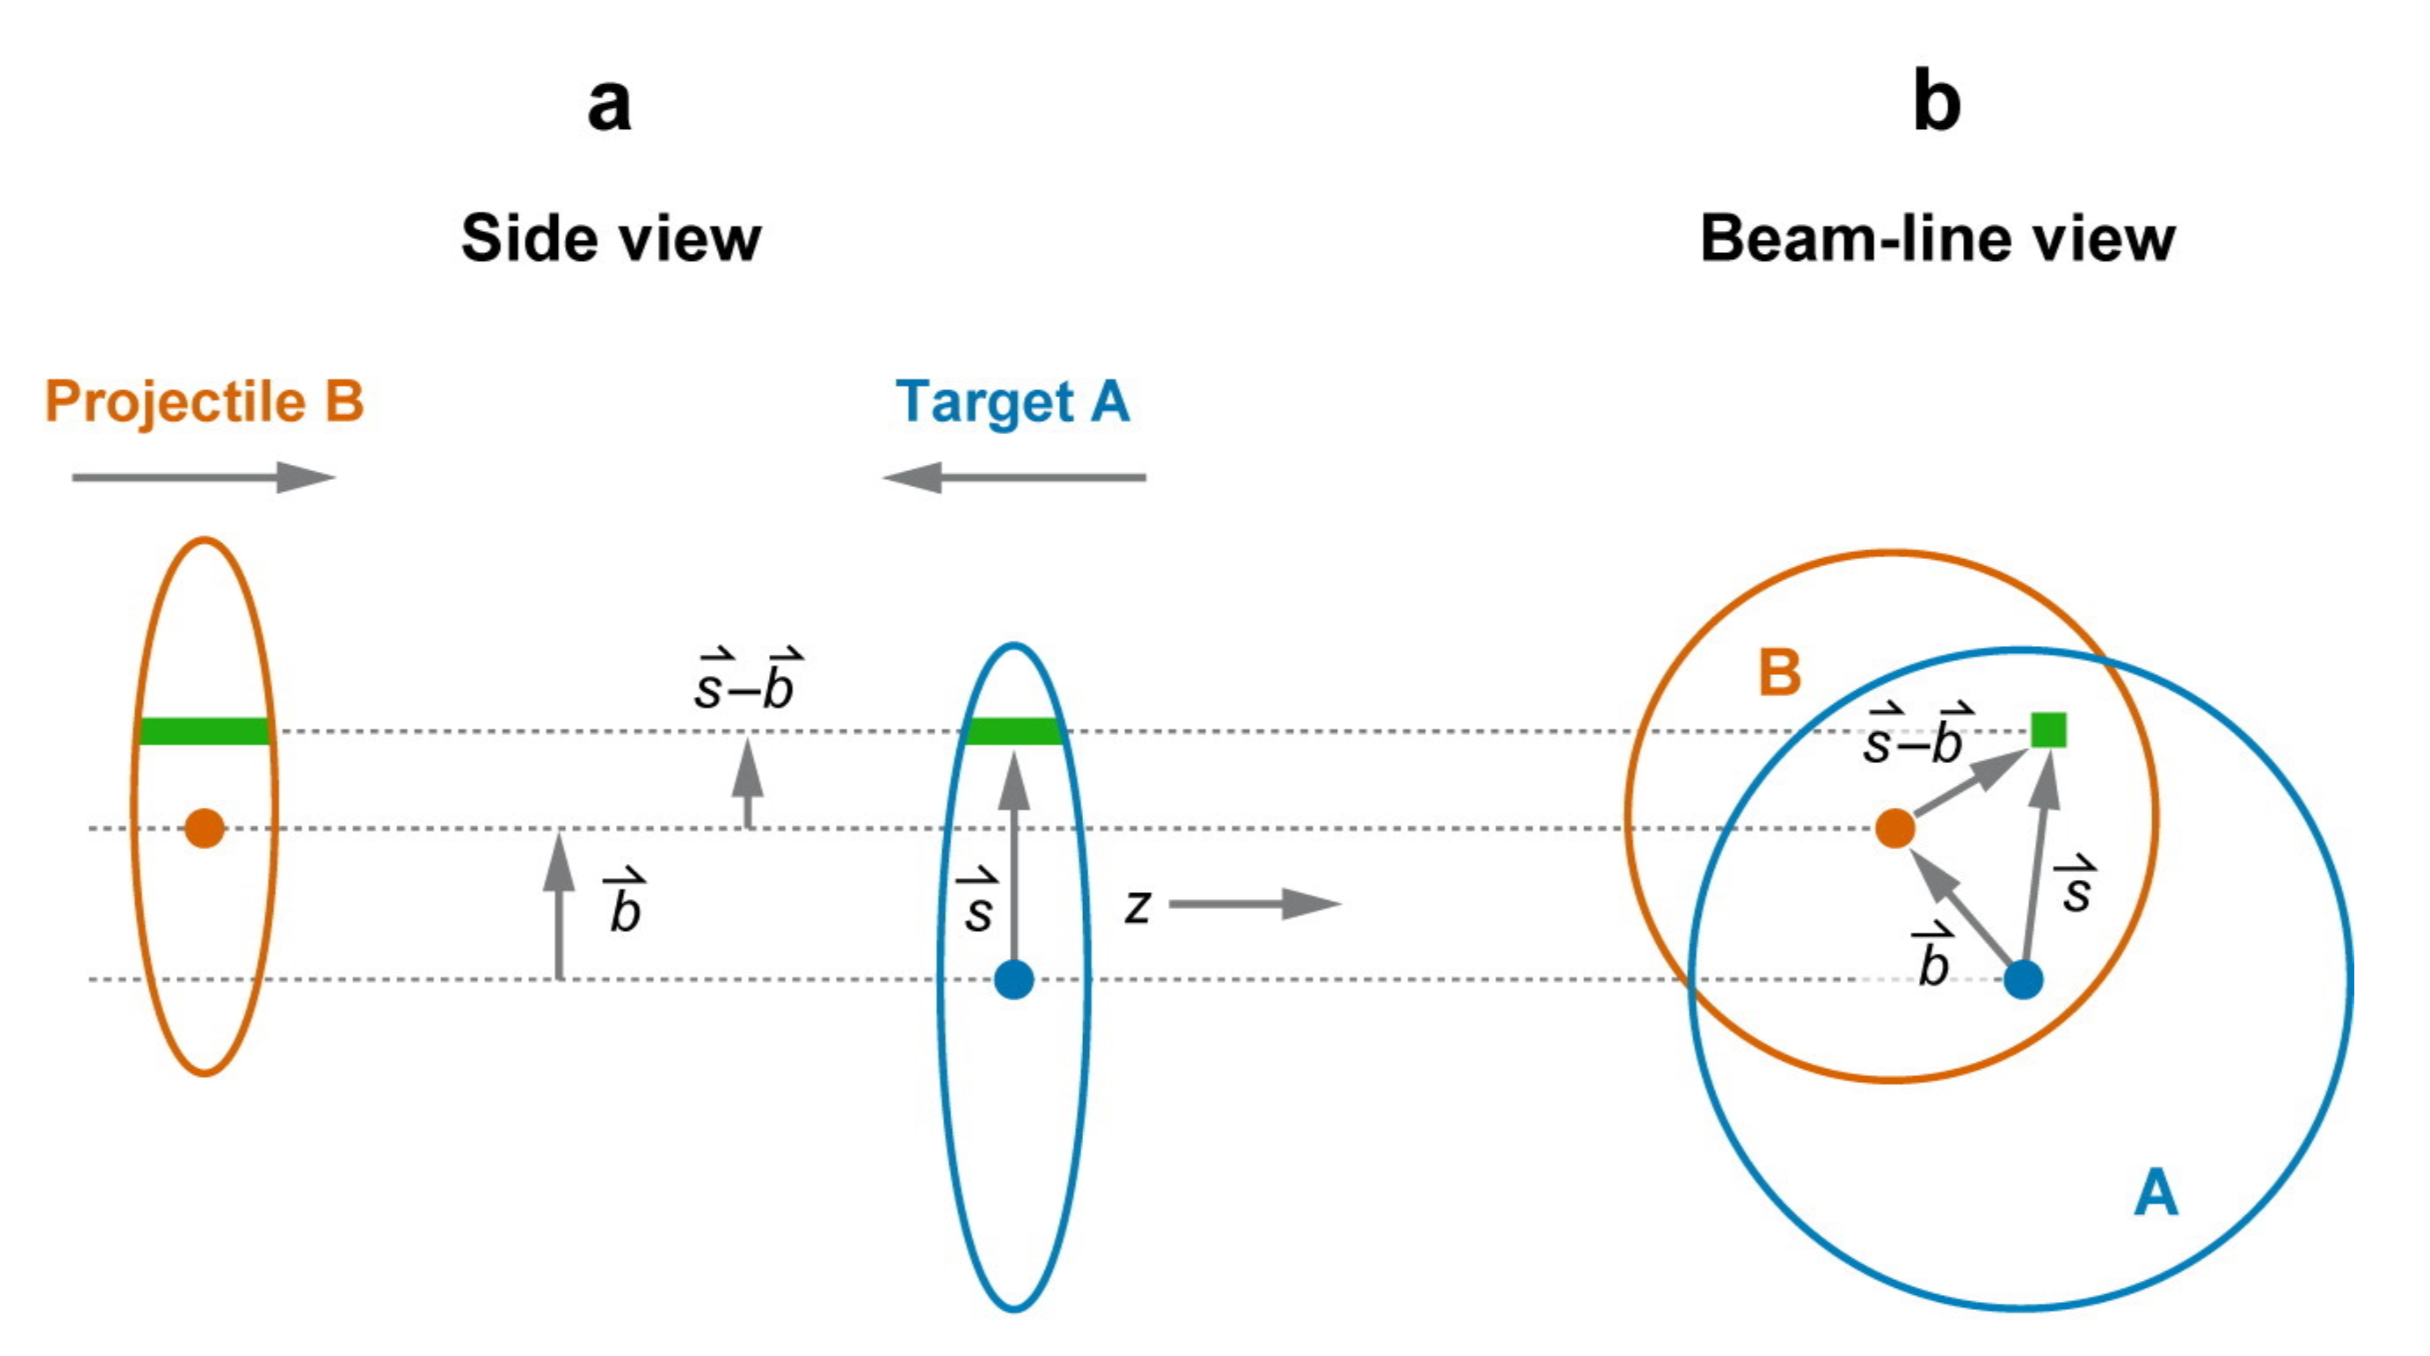
\includegraphics[width=0.9\textwidth]{gfx/glauber}
	\caption{Sketch of the longitudinal and transverse view of an heavy ion collision taken from \cite{glauber}. In the side view, the colliding nuclei are squeezed to represent the Lorentz boost contraction due to their momentum.}
	\label{fig:glauber}
\end{figure}

Following the notation introduced in Figure \ref{fig:glauber} the nuclear overlap function for two colliding
nuclei (A and B) can be written as:
\begin{equation} \label{eq:overlap}
    T_{AB}(\vec{b}) = \int T_{A}(\vec{s})\,T_{B}(\vec{s}-\vec{b}) \,d^{2}s
\end{equation}
and represents the probability of finding a nucleon in both the colliding nuclei inside the 
overlap region in the transverse plane.
$T_{A}(\vec{s})$ and $T_{B}(\vec{s}-\vec{b})$ are the \textit{thickness functions} the A and B
nuclei.
They represent the probability of finding a nucleon in the unit transverse area located at 
$\vec{s}\xspace$ given the probability per unit volume $\rho(\vec{s},z)$:
\begin{equation} \label{eq:thickfunc}
    T(\vec{s}) = \int \rho(\vec{s},z) \,dz.
\end{equation}




% Then, the probability of observing an interaction between two nucleons located in the overlap region is defined as the product of the nuclear overlap function and the total in- elastic cross section between two nucleons σinel. As already introduced, each nucleon does not deflect its trajectory after the interaction with another nucleons. As a consequence each nucleon can participate in more than one binary collision and the probability of having n binary collisions between the nuclei A and B, having A and B nucleons respectively, can be computed using the binomial statistics:
